%%%%%%%%%%%%%%%%%%%%%%%%%%%%%%%%%%%%%%%%%%%%%%%%%%%%%%
%SEC%%%%%%%%%%%%%%%%%%%%%%%%%%%%%%%%%%%%%%%%%%%%%%%%%%
\section{Implementação do Projeto}


%FRAME%%%%%%%%%%%%%%%%%%%%%%%%%%%%%%%%%%%%%%%%%%%%%%%
\begin{frame}{Implementação do Projeto}
O projeto é dividido em dois módulos:
\medskip
\begin{itemize}
    \item \textbf{Módulo 1}: Captura fotos, detecta faces e envia as faces para o segundo módulo
    \item \textbf{Módulo 2}: Verifica se a mesma face já foi analisada no passado e extrai características como idade, emoções e gênero
\end{itemize}
\end{frame}


%SUBSEC%%%%%%%%%%%%%%%%%%%%%%%%%%%%%%%%%%%%%%%%%%%%%%%
\subsection{Módulo 1}

%FRAME%%%%%%%%%%%%%%%%%%%%%%%%%%%%%%%%%%%%%%%%%%%%%%%
\begin{frame}{Módulo 1: Raspberry Pi}
\begin{itemize}
    \item É um computador de placa única de baixo custo
    \item Processador quad-core 64-bit de 1,4 GHz
    \item 1 GB de memória SDRAM
    \item Interface CSI para câmera
    \item Wifi e Ethernet
    \item Roda Linux ARM
\end{itemize}
\centerline{\noindent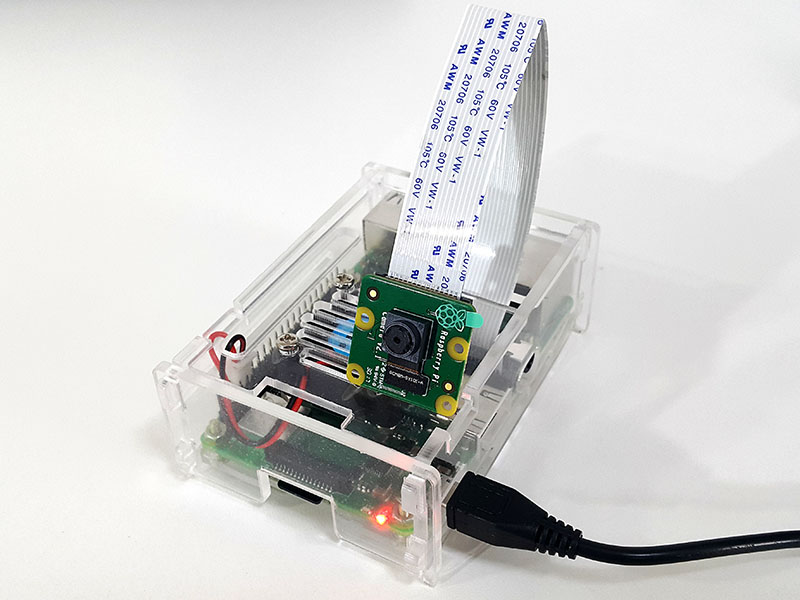
\includegraphics[width=0.45\linewidth]{raspberry.jpg}}
\end{frame}


%FRAME%%%%%%%%%%%%%%%%%%%%%%%%%%%%%%%%%%%%%%%%%%%%%%%
\begin{frame}{Módulo 1: Raspberry Pi}
\begin{itemize}
    \item Será instalado em pontos estratégicos da loja
    \item Realiza detecção utilizando o algoritmo de Viola-Jones implementado na OpenCV
    \item Envia apenas as imagens das faces para o segundo módulo para reduzir o tráfego de dados e as chamadas para a API
\end{itemize}
\end{frame}


%SUBSEC%%%%%%%%%%%%%%%%%%%%%%%%%%%%%%%%%%%%%%%%%%%%%%%
\subsection{Módulo 2}

%SUBSEC%%%%%%%%%%%%%%%%%%%%%%%%%%%%%%%%%%%%%%%%%%%%%%%
\subsubsection{Microsoft Face API}

%FRAME%%%%%%%%%%%%%%%%%%%%%%%%%%%%%%%%%%%%%%%%%%%%%%%
\begin{frame}{Módulo 2: Microsoft Face API}
\begin{itemize}
    \item Parte do Microsoft Azure Cognitive Services
    \item Realiza detecção, reconhecimento, agrupamento facial e extrai diversas outras características como emoção, idade, sexo, cor do cabelo, barba, maquiagem e uso de acessórios
    \item Grátis até 30000 transações por mês
    \item Aproximadamente R\$~3 a cada 1000 transações
\end{itemize}
\end{frame}

%FRAME%%%%%%%%%%%%%%%%%%%%%%%%%%%%%%%%%%%%%%%%%%%%%%%
\begin{frame}{Módulo 2: Microsoft Face API}
\begin{figure}[htbp]
%    \caption{Teste da Microsoft Face API}
    \label{fig:face_api_test1}
    \centering
    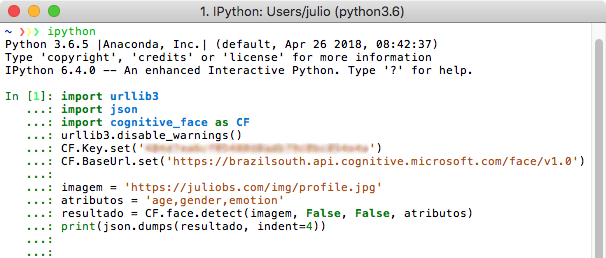
\includegraphics[height=0.8\textheight,width=\textwidth,keepaspectratio]{imagens/msft_face_api_json_1.png}
\end{figure}
\end{frame}


%FRAME%%%%%%%%%%%%%%%%%%%%%%%%%%%%%%%%%%%%%%%%%%%%%%%
\begin{frame}{Microsoft Face API}
\begin{figure}[htbp]
%    \caption{Teste da Microsoft Face API}
    \label{fig:face_api_test2}
    \begin{subfigure}[c]{0.48\textwidth}
    \centering
    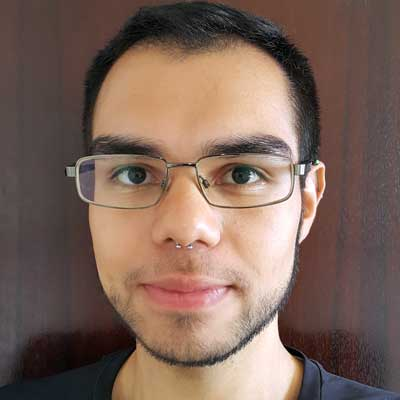
\includegraphics[height=\textheight,width=\textwidth,keepaspectratio]{imagens/profile.jpg}
    \end{subfigure}
    \begin{subfigure}[c]{0.48\textwidth}
    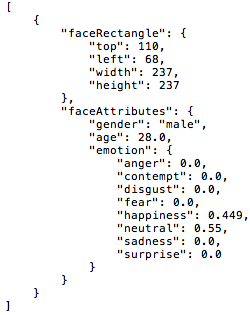
\includegraphics[height=\textheight,width=\textwidth,keepaspectratio]{imagens/msft_face_api_json_2.png}
    \end{subfigure}
\end{figure}
\end{frame}


%FRAME%%%%%%%%%%%%%%%%%%%%%%%%%%%%%%%%%%%%%%%%%%%%%%%
\begin{frame}{Microsoft Face API}
\begin{figure}[htbp]
    \caption{Python SDK para a Microsoft Face API}
    \centering
    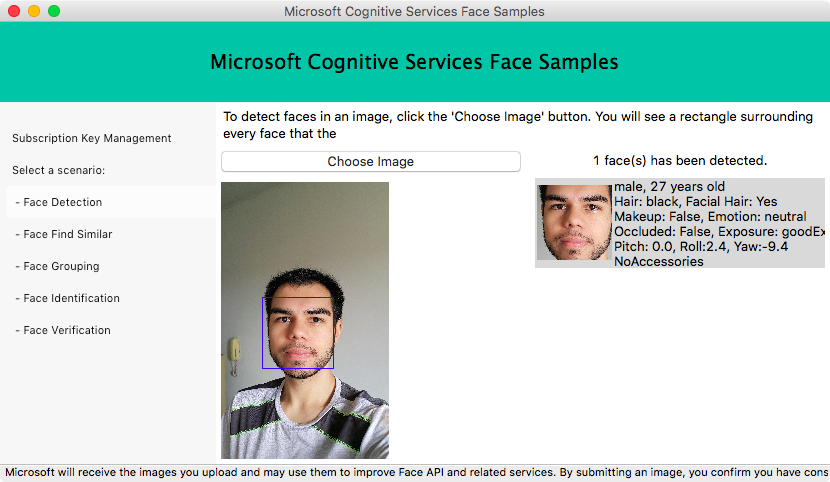
\includegraphics[width=0.8\linewidth]{imagens/msft_face_api_test.png}
\end{figure}
\end{frame}